\begin{figure}[htbp]
    \centering
    \resizebox{0.92\textwidth}{!}{%
    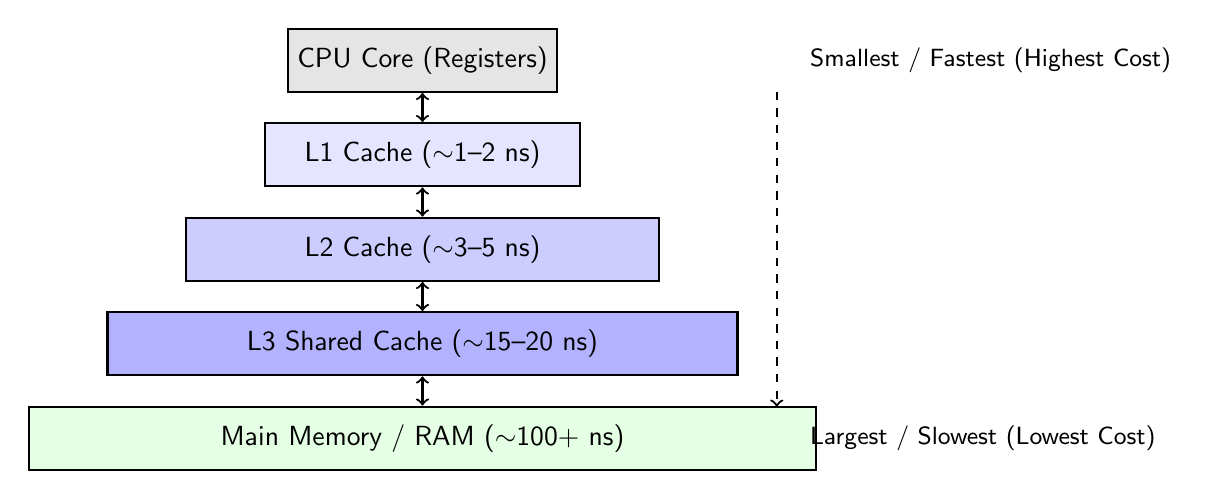
\begin{tikzpicture}[
        level/.style={rectangle, draw=black, thick, text centered, font=\sffamily, minimum height=0.8cm},
        core/.style={level, fill=gray!20, minimum width=2.5cm},
        l1/.style={level, fill=blue!10, minimum width=4cm},
        l2/.style={level, fill=blue!20, minimum width=6cm},
        l3/.style={level, fill=blue!30, minimum width=8cm},
        mem/.style={level, fill=green!10, minimum width=10cm},
        arrow/.style={<->, thick}
    ]
        % Nodes
        \node[core] (CPU) at (0, 0) {CPU Core (Registers)};
        \node[l1] (L1) at (0, -1.2) {L1 Cache ($\sim$1--2 ns)};
        \node[l2] (L2) at (0, -2.4) {L2 Cache ($\sim$3--5 ns)};
        \node[l3] (L3) at (0, -3.6) {L3 Shared Cache ($\sim$15--20 ns)};
        \node[mem] (RAM) at (0, -4.8) {Main Memory / RAM ($\sim$100+ ns)};

        % Arrows
        \draw[arrow] (CPU.south) -- (L1.north);
        \draw[arrow] (L1.south) -- (L2.north);
        \draw[arrow] (L2.south) -- (L3.north);
        \draw[arrow] (L3.south) -- (RAM.north);

        % Annotations
        \node[anchor=west, font=\sffamily\small] at (4.8, 0) {Smallest / Fastest (Highest Cost)};
        \node[anchor=west, font=\sffamily\small] at (4.8, -4.8) {Largest / Slowest (Lowest Cost)};
        \draw[->, thick, dashed] (4.5, -0.4) -- (4.5, -4.4);
    \end{tikzpicture}%
    }
    \caption{CPU memory hierarchy illustrating the explicit size-latency tradeoff. Faster layers are closer to the execution core but exponentially smaller in capacity.}
    \label{fig:cache_hierarchy}
\end{figure}
